\chapter{Нейросетевой метод управления на основе Актор-Критик обучения с подкреплением} \label{chapt3}

\section{Классификация ИНС} \label{sect3_1}

\subsection{Сети прямого распространения} \label{subsect3_1_1}

\subsection{Рекуррентные сети} \label{subsect3_1_2}
Сигнал с выходных нейронов или нейронов скрытого слоя частично передается обратно на входы нейронов входного слоя (обратная связь). Рекуррентная сеть Хопфилда «фильтрует» входные данные, возвращаясь к устойчивому состоянию и, таким образом, позволяет решать задачи компрессии данных и построения ассоциативной памяти. Частным случаем рекуррентных сетей являются двунаправленные сети. В таких сетях между слоями существуют связи как в направлении от входного слоя к выходному, так и в обратном. Классическим примером является Нейронная сеть Коско.

\section{Рекуррентный Критик} \label{sect3_2}

\section{Программное средство} \label{sect3_3}

\section{Экспериментальные исследования} \label{sect3_4}

\subsection{Управление машиной Дубинса в задаче преследования} \label{subsect3_3_1}

\begin{equation}
\label{eq:3_3_1p1}
\left\{
\begin{alignedat}{2}
\frac{dx}{dt}=v\cdot \cos (\phi ) \\
\frac{dy}{dt}=v\cdot \sin (\phi ) \\
\frac{d\phi}{dt}=\frac{\pi}{2}(u_{rm}-u_{lm}) \\
v=0.5(u_{rm}-u_{lm})
\end{alignedat}
\right.
\text{где}
\left\{
\begin{alignedat}{2}
u_{rm}=[0,1]\\
u_{lm}=[0,1]
\end{alignedat}
\right.
\end{equation}

\subsection{Мультиагентное взаимодействие в задаче преследования} \label{subsect3_3_2}

\subsection{Управление настройками ПИ-регулятора в задаче управления двуосным прокатным станом} \label{subsect3_3_3}

\begin{figure}[ht] 
	\center
	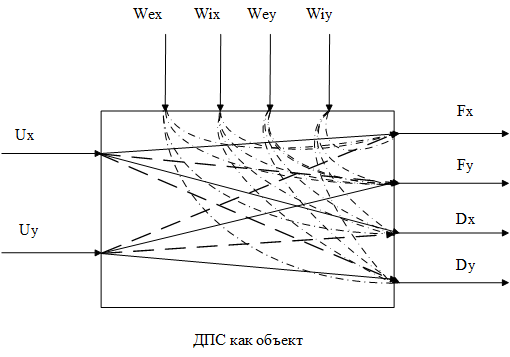
\includegraphics [scale=1] {dps}
	\caption{Представление ДПС как объекта} 
	\label{img:dps}  
\end{figure}

\begin{figure}[ht] 
	\center
	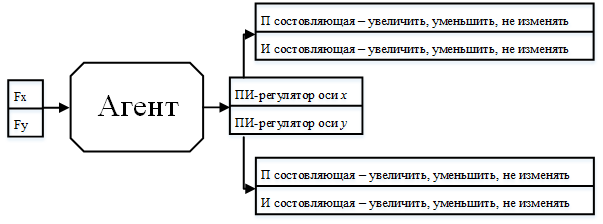
\includegraphics [scale=1] {agent_dps}
	\caption{Структурная схема работы Агента для управления ДПС} 
	\label{img:agent_dps}  
\end{figure}


\clearpage
\clearpage
